\section{Softwares de uso frecuente}

Existen muchos paquetes de simulaci\'on que implementan la teor\'ia del 
funcional de densidad. Estos paquetes de simulaci\'on se diferencian por el 
conjunto de funciones base que utilizan, los tipos de pseupotenciales que 
admiten y las propiedades que pueden calcular, entre otros aspectos. A 
continuaci\'on se presenta una lista de algunos paquetes de simulaci\'on 
relevantes.

\begin{itemize}
    \item \textbf{VASP:}  Es un paquete de simulaci\'on para modelamiento de 
    materiales a escala at\'omica como c\'alculos de estructura electr\'onica y 
    din\'amica molecular mec\'anico-cu\'antica a partir de primeros principios. 
    Implementa la teor\'ia del funcional de densidad, funcionales h\'ibridos, 
    teor\'ia de perturbaci\'on y el m\'etodo de funciones de Green. Adem\'as 
    utiliza pseudopotenciales, m\'etodo del proyector de ondas aumentadas y 
    ondas planas.
    \item \textbf{WIEN2k:} Es un paquete de simulaci\'on que permite realizar 
    c\'alculos de estructura electr\'onica de s\'olidos usando la teor\'ia del 
    funcional de densidad. Implementa el m\'etodo de ondas planas aumentadas 
    linealizadas m\'as orbitales locales (LAPW + lo) y tambi\'en es capaz de 
    considerar efectos relativistas.
    \item \textbf{ABINIT:} Es un paquete de simulaci\'on para c\'alculos de 
    estructura electr\'onica que implementa la teor\'ia del funcional de 
    densidad con pseudopotenciales o wavelets. Adem\'as implementa la teor\'ia 
    de perturbaciones y la teor\'ia del funcional de densidad dependiente del 
    tiempo.
    \item \textbf{Quantum ESPRESSO:} Es una suite de paquetes de simulaci\'on 
    para c\'alculos de estructura electr\'onica que implementa la teor\'ia del 
    funcional de densidad utilizando pseudopotenciales y ondas planas. Adem\'as 
    implementa la teor\'ia del funcional de densidad dependiente del tiempo. 
    Este es el software que se utiliza en el presente estudio.
\end{itemize}


\section[C\'alculos de estructura electr\'onica usando la suite Quantum \\
ESPRESSO]{C\'alculos de estructura electr\'onica usando la suite Quantum 
ESPRESSO}

El siguiente diagrama muestra el proceso que se sigue en un c\'alculo autoconsistente convencional con Quantum ESPRESSO.

\begin{figure}[H]
	\centering
	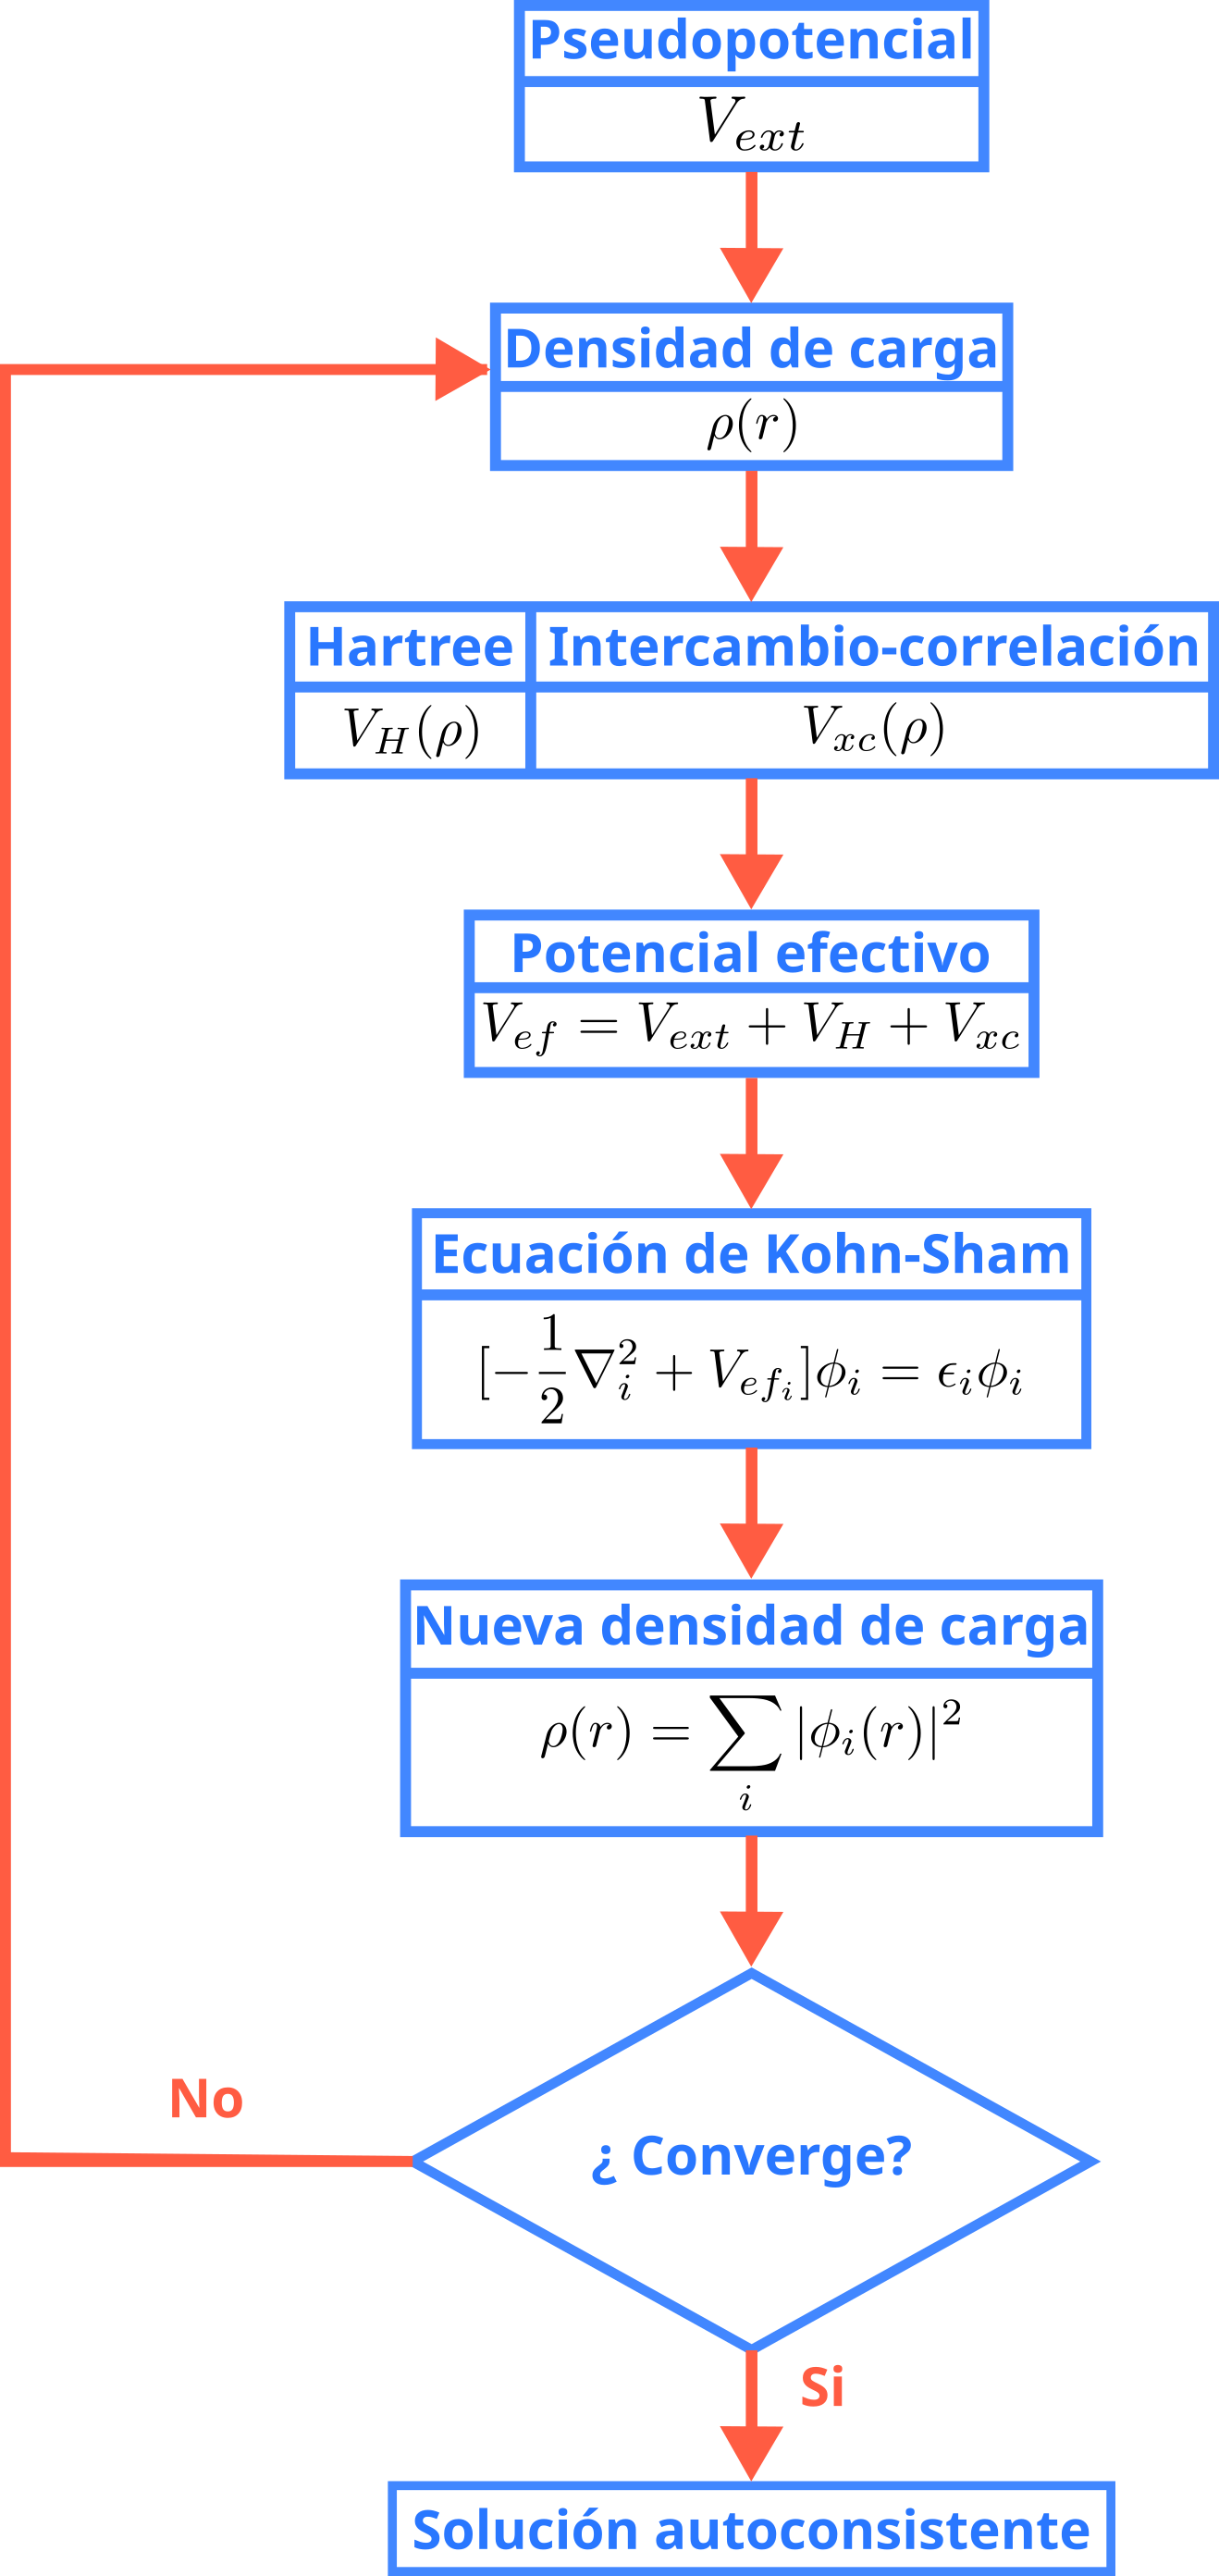
\includegraphics[width=0.4\textwidth]{contenido/calculos_computacionales/calculos_autoconsistentes/img_autoconsistente/BucleAutoconsistente.png}
	\caption[Diagrama del proceso de c\'alculo de campo 
	autoconsistente]{Diagrama del proceso de c\'alculo de campo 
		autoconsistente.}
\end{figure}

Quantum ESPRESSO se encuentra formado por varios programas que cumplen una 
gran variedad de funciones. En el presente trabajo se utilizaron 
los siguientes programas espec\'ificos:

\begin{itemize}
    \item pw.x : Realiza el c\'alculo de autoconsistencia y el c\'alculo de 
    bandas de energ\'ia.
    \item bands.x : Extrae la informaci\'on correspondiente a cada una 
    de las bandas de energ\'ia, desde los archivos de salida producidos por pw.x
    \item projwfc.x : Realiza el c\'alculo de densidad de estados total y 
    parcial.
    \item plotband.x : Grafica las bandas de energ\'ia a partir de lo obtenido 
    con bands.x
    \item pp.x : Extrae los datos correspondientes a la densidad de carga, a 
    partir de lo obtenido con pw.x
    \item plotrho.x : Grafica la densidad de carga a partir de lo obtenido con 
    pp.x
\end{itemize}

\noindent Adem\'as de la suite Quantum ESPRESSO se utilizaron otros programas 
que se especifican a continuaci\'on.

\begin{itemize}
    \item VESTA : Generaci\'on y visualizaci\'on de la estructura at\'omica 
    utilizada en la simulaci\'on
    \item XCrySDen : Generaci\'on del camino de puntos K para el c\'alculo de 
    la estructura de bandas de energ\'ia. Adem\'as permite revisar que la 
    estructura del archivo de control de Quantum ESPRESSO sea el adecuado.
    \item Veusz : Programa para generar gr\'aficas
    \item Scripts : Scripts desarrollados espec\'ificamente para el 
    presente trabajo en python y shell para automatizar procesos.
\end{itemize}

\noindent El proceso de simulaci\'on con la suite Quantum ESPRESSO seguido en 
el presente trabajo puede ser separado en tres secciones.

\begin{itemize}
    \item Preprocesamiento.
    \item Simulaci\'on.
    \item Postprocesamiento.
\end{itemize}

\noindent Cada una de estas secciones se conforma de una serie de pasos que 
se listan 
a continuaci\'on.

\begin{enumerate}
    \item \textbf{Preprocesamiento:}
    \begin{itemize}
        \item Optimizaci\'on de la energ\'ia de corte.
        \item Optimizaci\'on del n\'umero de puntos K.
        \item Generacion de las estructuras cristalinas con los diferentes 
        arreglos antiferromagn\'eticos
        \item C\'alculo del par\'ametro U de Hubbard.
        \item Relajaci\'on de las estructuras cristalinas.
    \end{itemize}
    \item \textbf{Simulaci\'on:}
    \begin{itemize}
        \item C\'alculo autoconsistente con pw.x
        \item C\'alculo de la densidad de carga con pp.x
        \item C\'alculo no autoconsistente con pw.x
        \item C\'alculo de la densidad de estados total y parcial con 
        projwfc.x
        \item C\'alculo de las bandas de energ\'ia con pw.x
        \item Obtenci\'on de los datos de cada una de las bandas de 
        energ\'ia con bands.x
    \end{itemize}
    \item \textbf{Postprocesamiento:}
    \begin{itemize}
        \item Procesamiento de los archivos obtenidos con projwfc.x 
        utilizando el script de python suma\_pdos.py para luego graficar 
        las densidades de estado.
        \item Procesamiento de los archivos obtenidos con bands.x 
        utilizando el script de python banda\_plot.py para luego graficar 
        las bandas.
    \end{itemize}
\end{enumerate}

